\documentclass{article}
\usepackage[utf8]{inputenc}
\usepackage[main=catalan, english]{babel}
\usepackage{graphicx}
\usepackage{wrapfig}
\usepackage{multicol}
\usepackage{blindtext}
\usepackage{wallpaper}

\RequirePackage{fontspec}
\defaultfontfeatures{ Ligatures={TeX}, Path = {./fonts/}, }
\newfontfamily\Cartamagna{CartaMagna.ttf}
\graphicspath{ {./images/} }
\begin{document}
\title{El monestir}
\begin{titlepage}
    \centering
    \vspace*{2cm}
    \Huge
    \ThisLRCornerWallPaper{1.0}{masia2.png}
    \resizebox{100mm}{!}{\color[gray]{0}\Cartamagna El monestir}
    \vfill
    \vspace{0.8cm}
\end{titlepage}
\maketitle
\section{Pannagiri}
Pannagiri es el monasterio de los nagas, un lugar sagrado en la tradición budista.
\begin{wrapfigure}{r}{0.25\textwidth} %this figure will be at the right
    \centering
    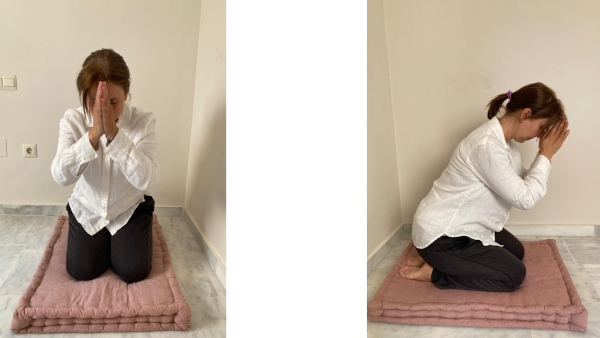
\includegraphics[width=0.25\textwidth]{vandami_woman.jpg}
\end{wrapfigure}
On the other side, if you are only interested on
certain values yhgfgdou can use the contour plot, you 
can use the contour plot, you can use the contour 
plot, you can use the contour plot, you can use 
the contour plot, you can use the contour plot, 
you can use the contour plot, like the one on the left.

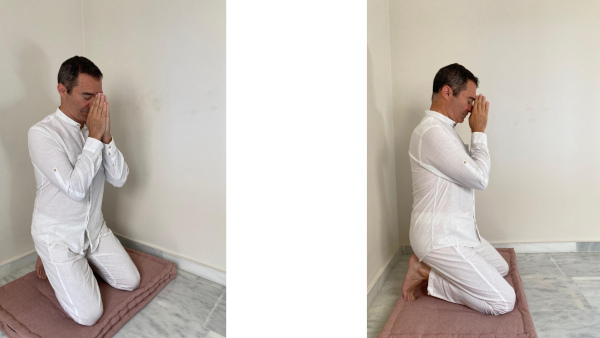
\includegraphics[width=5cm, height=4cm]{vandami_man.jpg}

On the other side, if you are only interested on 
certain values you can use the contour plot, you 
can use the contour plot, you can use the contour 
plot, you can use the contour plot, you can use the 
contour plot, you can use the contour plot, 
you can use the contour plot, 
like the one on the left.

\begin{wrapfigure}{r}{0.25\textwidth} %this figure will be at the right
    \centering
    \includegraphics[width=0.25\textwidth]{wave.png}
\end{wrapfigure}

\foreignlanguage{english}{\Blindtext}


\foreignlanguage{english}{dsaghfdsga}



\begin{multicols*}{2}
[
\section{First Section}
All human things are subject to decay. And when fate summons, Monarchs must obey.
]
\Blindtext
\end{multicols*}

\begin{multicols}{2}
[
\section{Nuestra Tradicion}
All human things are subject to decay. And when fate summons, Monarchs must obey.
]
Hello, here is some text without a meaning.  This text should show what 
a printed text will look like at this place.
\begin{wrapfigure}{l}{0.7\linewidth}
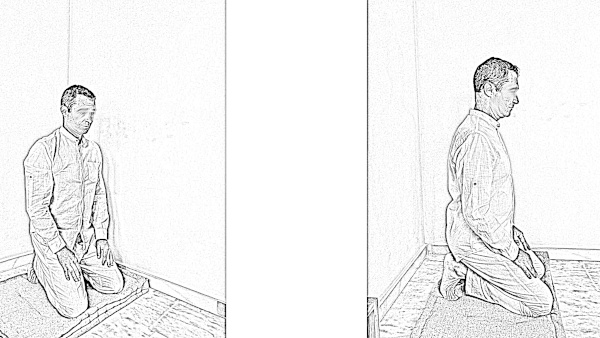
\includegraphics[width=\linewidth]{prep-man-ai.jpg}
\caption{This is the Overleaf logo}
\end{wrapfigure}
If you read this text, you will get no information.  Really?  Is there 
no information?  Is there.
\foreignlanguage{english}{\blindtext
\vfill


}

\columnbreak
\blindtext
This will be in a new column, here is some text without a meaning.  This text 
should show what a printed text will look like at this place.

If you read this text, you will get no information.  Really?  Is there 
no information?  Is there...
\end{multicols}

\end{document}
